\chapter{Summary}
\label{summary}


\section{Tracing star formation with ultraviolet flux: results from sub-kpc regions}

In this study, we have derived the recent ($< 500\myr$) SFHs of 33
UV-bright regions in M31 using optical HST observations from PHAT. The regions
were defined by \citetalias{Kang:2009} based on GALEX \fuv{} surface brightness and
have areas ranging from $8 \times 10^3$ to $1.5 \times 10^6\pc^2$. We
used the SFH code MATCH to fit the CMDs of the regions and measure their the
SFHs based on the resolved stars from the PHAT photometry. We modeled the
extinction in the regions using a foreground parameter and a differential
parameter, which were optimized for each region to find the best-fit SFH.

We used FSPS to model both the intrinsic and reddened \fuv{} and \nuv{} magnitudes of
the regions based on their SFHs. The differences between the modeled reddened
and the observed \fuv{} magnitudes, $\fuvsfh - \fuvobs$, followed a
normal distribution with $\mu=0.09$ and $\sigma=0.3$. On average, the
\fuvsfh{} values were consistent with the \fuvobs{}
values, confirming the reliability of the SFHs, our extinction model, and the
\citet{Cardelli:1989} extinction curve. We attribute the scatter in the flux
ratios to the assumption made by FSPS that the IMF is fully populated while the
actual distribution of stellar masses becomes more discrete as smaller regions
are considered.

The observed, extinction-corrected \fuv{} magnitudes were converted into SFRs,
\sfrfuv{}, using the \fuv{} flux calibration from \citet{Kennicutt:1998}
with updates by \citet{Hao:2011} and \citet{Murphy:2011}. We also derived the mean
SFRs for the last $100\myr$ of the SFHs, \sfroneh{}. The $\sfrfuv / \sfroneh$
ratios were log-normally distributed with $\mu=0.2$
and $\sigma=0.4$. Overall, the \sfrfuv{} values were consistent with
the \sfroneh{} values, though a small amount of the
offset was attributable to inconsistencies with the metallicity assumed by the
flux calibration.

The intrinsic modeled \fuv{} magnitudes were also converted into SFRs,
\sfrfuvz{}, which were free from biases due to extinction
corrections and IMF sampling. The log-normal for the
$\sfrfuvz / \sfroneh$ ratios had $\mu=0.1$
and $\sigma=0.3$, indicating that assuming a constant SFR (implicit in the flux
calibration) for regions with highly variable SFHs is an important source of
scatter. We conclude that the total scatter in the $\sfrfuv / \sfroneh$ ratio
is due to the assumptions of a full IMF and a
constant SFR in regions where discrete sampling of the IMF and high variability
in the SFHs are important. Combined, these effects result in a factor of 2.5
uncertainty in the \fuv{}-based SFRs. Although there is a significant lack of
regions in our sample with areas between $10^5$ and $10^6\pc^2$, we
estimate that discrete IMF sampling and SFH variability become important below
$10^5\pc^2$, or scales of a few hundred pc.

Ages and masses were derived for the regions by \citetalias{Kang:2009} from
observed $\fuv - \nuv$ color and \fuv{} luminosity, using the assumption that
the regions are SSPs. By comparing the ages to the SFHs, we found that most of
the regions are entirely inconsistent with the SSP assumption. Furthermore, the
ages often did not correspond to the main episodes of SF, and the masses were
discrepant with the masses integrated from the SFHs by up to 2 orders of
magnitude. These results call into question the practice of deriving ages and
masses for populations that are not confirmed SSPs.

We identified SSP-like regions as regions which formed 90\% or more of their
mass over the past $100\myr$ in a single age bin of their SFH. These
regions accounted for 18\% of our sample (6 of 33). Among this subset, we found
discrepancies of $10\myr$ in the ages and a factor of $3-4$ in the
masses derived from UV flux, most likely due to systematics in metallicity and
extinction. We propose that these discrepancies represent realistic
uncertainties in the SSP ages and masses, though the limited number of SSP-like
regions in our sample makes the uncertainties difficult to determine. Finally,
identification of the SSP-like regions was not possible from integrated \fuv{}
flux.



\section{Modeling ultraviolet flux on sub-kpc scales and galactic scales simultaneously}

We have used star formation histories (SFHs) to model the spectral energy
distributions (SEDs) of over 9000 sub-kpc regions in M31 and produce detailed
maps of synthetic UV flux across the entire area covered by the Panchromatic
Hubble Andromeda Treasury (PHAT). This work is an extensive follow-up to the
analysis of \citet{Simones:2014}, which involved only 33 ultraviolet
(UV)-bright regions from a small portion of the galaxy. The SFHs were derived
by \citet{Lewis:2014}\ using \acsb{} and \acsi{} photometry from the PHAT
survey. Both intrinsic and attenuated SEDs were derived from the SFHs using the
Flexible Stellar Population Synthesis (FSPS) code. These were convolved with
the Galaxy Evolution Explorer (GALEX) \fuv{} and \nuv{} response curves to
obtain the synthetic intrinsic fluxes, \fxsfhz{}, as well as the synthetic
attenuated fluxes, \fxsfh{}. All of the flux values were then assembled into an
overall map, or mosaic, using Montage. The mosaic pixels corresponded to
physical areas of $4.4\times 10^4\pc^2$. We constructed corresponding maps for
the observed flux, \fxobs{}, using GALEX Deep Imaging Survey (DIS) images.

The \fxsfh{} maps agreed with the \fxobs{} maps very well with respect to the
broad morphology of M31, faithfully reproducing all of the main features
brighter than $\sim 10^{-15}\uflambda$. We found the log ratios of \fxsfh{} to
\fxobs{} to be log-normally distributed with $\mu = 7.62\times 10^{-3}$ and
$\sigma = 2.37\times 10^{-1}$ for \fuv{}, and $\mu = -1.03\times 10^{-1}$ and
$\sigma = 1.59\times 10^{-1}$ for \nuv{}. The median flux ratios were 1.02 in
\fuv{} and 0.79 in \nuv{}, with 68\% confidence limits of 0.59 and 1.76
(\fuv{}) and 0.55 and 1.14 (\nuv{}). In both filters, the median ratio was
within the confidence interval of 1, indicating that \fxsfh{} was consistent
with \fxobs{} on average. Due to the small pixel areas, the primary source of
the variance in the log flux ratios was most likely related to incomplete
sampling of the IMF.

We found no obvious trends in the flux ratios with respect to environment,
except for in the faintest, off-arm areas of the M31 where the variances in the
flux ratios were noticeably larger. We conclude that fluxes may be successfully
modeled from SFHs for any population in environments similar to M31. For our
sub-kpc regions, we estimate the synthetic flux uncertainties to be
$+\!0.74/\!-\!0.43$ and $+\!0.35/\!-\!0.24$ in \fuv{} and \nuv{}, respectively.
Results from previous work on UV-bright regions by \citet{Simones:2014} were
consistent with our results.

The overall agreement between the observed and synthetic fluxes is remarkable
considering that our flux modeling procedure was dependent on several key
assumptions. Specifically, we assumed an IMF, models describing stellar spectra
and evolution, and an extinction model as well as an extinction curve. These
form the foundation for much research in astronomy and encompass our current
best understanding of stellar astrophysics and star formation. It is reassuring
that we can use all of this knowledge to successfully recreate detailed maps of
a galaxy from photometry in just two optical bands.

We used flux calibrations from \citet{Kennicutt:1998} with updates by
\citet{Hao:2011} and \citet{Murphy:2011} to estimate SFRs based on observed UV
flux, \sfrx{}. The \fxobs{} maps were first corrected for extinction using the
synthetic attenuated and intrinsic fluxes. We also calculated the $100\myr$
mean SFR from the SFHs, \sfroneh{}. We found that the faintest areas of M31 had
the highest ratios of \sfrx{} to \sfroneh{} and formed a linear tail feature in
plots of the SFR ratio versus \sfroneh{}. These tails were the result of a
distinct breakdown of the linear relationship between flux and SFR which
underpins the flux calibration method. We estimated a conservative threshold of
$\sfr \sim 10^{-5}\msun\yr^{-1}$ below which flux calibration should not be
used.

For the pixels above this threshold, we found the SFR ratios to be log-normally
distributed with $\mu = -2.46\times 10^{-1}$ and $\sigma = 2.61\times 10^{-1}$
for \fuv{}, and $\mu = 9.27\times 10^{-2}$ and $\sigma = 2.33\times 10^{-1}$
for \nuv{}. The median ratios are 0.57 (\fuv{}) and 1.24 (\nuv{}), with 68\%
confidence limits of 0.31 and 1.04 (\fuv{}) and 0.72 and 2.12 (\nuv{}),
indicating that \sfrx{} is consistent with \sfroneh{} on average. As with the
flux ratios, incomplete sampling of the IMF was the main source of the variance
in the SFR ratios. We also considered deviations from solar metallicity as well
as SFH variability, and found that they were far less important for the overall
variances in the SFR ratios than IMF sampling.

Other than the faintest, off-arm areas which responsible for the tail feature
in the SFR ratio distributions, there were no found no obvious trends in the
SFR ratios with respect to environment. We determine that the flux calibration
method is safely applicable to environments similar to M31, \emph{but only as
long as the resulting \sfr{}s are greater than $\sim 10^{-5}\msun\yr^{-1}$}. We
estimate the SFR uncertainties for our sub-kpc regions to be
$+\!0.47/\!-\!0.26$ (\fuv{}) and $+\!0.88/\!-\!0.52$ (\nuv{}) times the true,
underlying $100\myr$-mean SFR. The \sfrfuv{} uncertainty is rather less than
the $+\!2.15/\!-\!0.88$ uncertainty previously found by \citet{Simones:2014}.

We also measured global SFRs for the entire PHAT survey area. The global
\sfroneh{} value was $0.30\msun\yr^{-1}$, while the UV flux-based values were
$\sfrfuv = 0.22\msun\yr^{-1}$ and $\sfrnuv = 0.43\msun\yr^{-1}$. The flux-based
global SFRs are consistent with the global \sfroneh{} value to within the
uncertainties derived from the SFR maps. However, the variances in the SFR
ratios due to IMF sampling is expected to decrease for larger areas, so our
estimated uncertainties should be considered firm upper limits when applied to
galaxies. The global SFR ratios (flux-based to mean) are 0.73 and 1.43 for
\fuv{} and \nuv{}, respectively. Why these ratios are larger than the median
ratios above is not yet understood.



\section{Future work}

\subsection{More precise quantification and attribution of uncertainties}

The two studies presented here share some key similarities. First, they both
show the importance of stochasticity in both the modeling of observed flux and
in the estimation of SFRs. The large variations in the derived fluxes and SFRs
with respect to their expected values due to incomplete IMF sampling
significantly limited the precision to which each could be determined (more so
in Chapter \ref{m31flux} than Chapter \ref{uv_regions}). While arguably not as
important when considering galaxies as a whole, care must be taken when
analyzing and comparing the flux content of stellar populations on much smaller
scales.

Second, the work here demonstrates that sample design has a critical influence
on the results of any given study. For example, the sample studied in Chapter
\ref{uv_regions} only included only a small subset of the UV-bright regions in
one small portion of M31. It was not until the full PHAT dataset was considered
in Chapter \ref{m31flux} that the unexpected nonlinearity between UV flux and
SFR was found for SFRs below $\sim 10^{-5}\msun\yr^{-1}$.

The PHAT photometry and the SFHs derived from it make up such an incredibly
rich dataset that the work presented in this thesis is far from complete. An
interesting possibility for the future is to investigate more deeply the
variance in the flux and SFR ratios discussed in Chapter \ref{m31flux}.
Specifically, an in-depth CMD analysis of the stellar populations behind each
map pixel would lead to a better understanding of the degree to which IMF
sampling really affects the total uncertainty in each data point. A simple
census of the main sequence stars in each CMD would be a good starting point. A
follow-up analysis involving models of stellar populations with different
numbers of stars would help to determine the inherent uncertainty that can be
expected for the fluxes and SFRs derived in Chapter \ref{m31flux}. Any
discrepancies between the total variances observed in the data and the expected
contribution from incomplete IMF sampling alone could provide clues about other
possible sources of uncertainty not yet recognized.


\subsection{Putative flux ratio and SFR ratio outliers}

A thorough investigation of the putative outliers in the flux and SFR ratio
distributions would be another interesting topic for the future. It is unknown
at this time whether the most discrepant data points are simply extreme cases
of the same dispersion affecting all of the data, or if such points are genuine
outliers. Similar to the analysis of IMF sampling proposed above, the simplest
places to look for clues are the CMDs. It is certainly possible that a small
subset of the putative outliers are genuine due to the contamination of
foreground stars in their CMDs. Once identified, such stars could be cleaned
from the photometry to improve the SFHs of \citet{Lewis:2014}, and presumably
the synthetic fluxes and flux-based SFR estimates as well, leading to a more
accurate characterization of the uncertainties involved in flux modeling and
SFR estimation. The large discrepancies in the flux-based SFRs may also be
explained by high variability in the derived SFHs. While such variability was
not found to be important for M31 overall as discussed in Chapter
\ref{m31flux}, it was found in Chapter \ref{uv_regions} to be a significant
source of uncertainty in the flux-based SFRs of UV-bright regions. The only
definitive answer to whether the SFR outliers are caused by non-constant SFHs
is to look at their SFHs directly.


\subsection{Synthetic flux and flux-based SFR uncertainties as a function of scale}

Chapters \ref{uv_regions} and \ref{m31flux} looked at flux modeling and SFR
estimation on both sub-kpc scales and galactic scales. These represent the
endpoints of a wide range of sizes, yet none of the intermediate scales (e.g.,
$\sim 1$ to $10\kpc$) have been considered. It was shown in Chapter
\ref{uv_regions} that the uncertainties in both the synthetic fluxes and the
estimated SFRs decreased with increasing area, presumably due to more complete
IMF sampling and an overall averaging out of SFH variations. However, the
sample was severely limited and it was not possible in that study to examine
the trend for scales larger than $\sim 1\kpc$. In contrast, the maps presented
in Chapter \ref{m31flux} are an ideal dataset for exploring quantitatively how
the uncertainties in the synthetic fluxes and the flux-based SFRs decrease with
area. By grouping the map pixels together into successively larger regions, a
complete distribution of sizes ranging from sub-kpc through galactic scales can
be studied.


\subsection{Synthetic flux and flux-based SFR uncertainties as a function of environment}

Another possibility is to group the map pixels by surface brightness and
environment (or radius), as shown in the prototype sample in Figure
\ref{fig:proto}. This would result in a two-dimensional sample where each
region represents a much larger fraction of the total survey area than a single
pixel, tempering the uncertainties due to IMF sampling. It would therefore be
possible to investigate more precisely how different conditions within M31
influence the outcome of flux modeling and the agreement between flux-based
SFRs and the derived SFHs. It might then be possible to use the resulting
environment-specific uncertainties for UV flux analyses of more distant
galaxies for which resolved stars are not available.


\begin{figure}
\centering
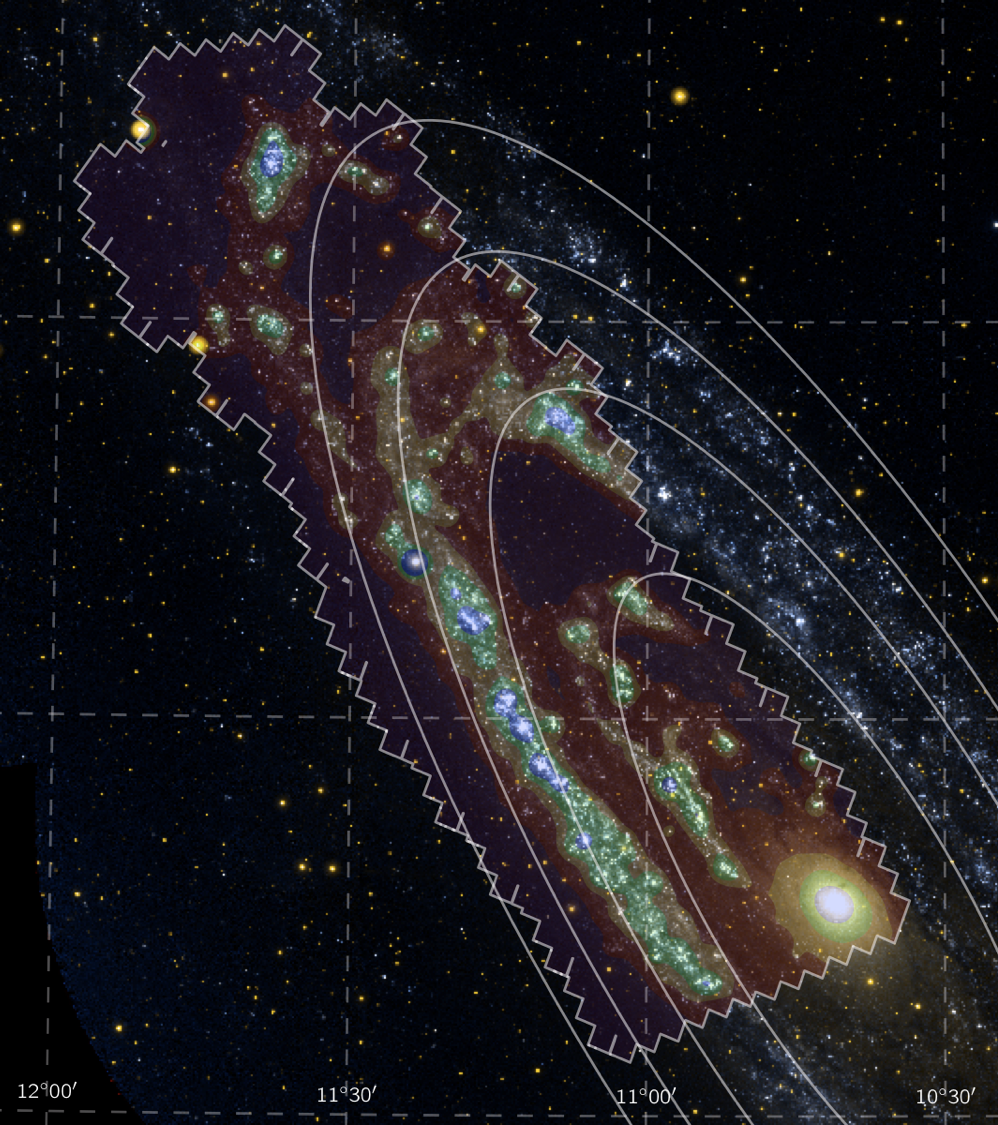
\includegraphics[scale=0.85]{prototype.pdf}
\caption[Two-dimensional prototype sample.]{Two-dimensional prototype sample
    for future investigation of the accuracy of flux modeling and flux-based
    SFR estimation as a function of both surface brightness and galactocentric
    radius. This example shows the PHAT survey divided into five levels of
    \fuv{} surface brightness (purple, red, orange, green, and blue shaded
    regions, from faintest to brightest) and again into five radial bins of
    approximately equal area.
}
\label{fig:mfx:dummy1}
\end{figure}


\subsection{Infrared flux as a test of dust emission models and as a SFR indicator}

Finally, the set of synthetic flux maps presented in Chapter \ref{m31flux} can
be extended to include maps for other instrument/filter combinations. Perhaps
the most interesting choice would be to model the flux in M31 as seen through
the $24\mu\mathrm{m}$ channel of the Spitzer Space Telescope. Developing such a
map would require an SED for the infrared (IR) dust emission in addition to the
stellar SED described in Chapter \ref{m31flux}. This would therefore present an
opportunity to test the accuracy of different dust emission models in M31,
e.g., the silicate-graphite-PAH model by \citet{Draine:2007}.

$24\mu\mathrm{m}$ flux is also conspicuous tracer of star formation and
therefore has been calibrated for predicting SFRs \citep[see the review by][and
references therein]{Kennicutt:2012}. The first interesting comparison with
respect to the work presented in Chapter \ref{m31flux} would be between the UV
flux-based SFRs and the $24\mu\mathrm{m}$ flux-based SFRs in terms of how well
they agree with the mean SFRs derived from the SFHs. So-called ``hybrid''
calibrations also exist, which predict SFRs using fluxes from multiple
wavelengths. In principle, hybrid calibrations are more robust than their
monochromatic counterparts because they account for more complex physics that
processes the observed light. For example, the combination of \fuv{} flux with
$24\mu\mathrm{m}$ flux accounts for both the direct starlight from massive
stars and the starlight that is absorbed by dust and reradiated in the IR. The
UV extinction correction is therefore built-in, in a sense, so the observed UV
and IR fluxes can be used directly without modification. Comparing a map of
hybrid $\fuv + 24\mu\mathrm{m}$ flux-based SFRs with the mean SFH-based SFRs
would be very interesting indeed, especially with respect to environments that
are particularly dusty versus those that are not.
